\begin{center}
\Huge
Trigonometriske funktioner og Pythagoras
\end{center}

\section*{Trigonometriske funktioner}
\stepcounter{section}

Vi har tidligere set, hvordan de trigonometriske funktioner $\sin$ og $\cos$ er defineret ud fra enhedscirklen. I dag skal vi se, hvordan vi definerer den trigonometriske funktion $\tan$, og så skal vi definere relationsformlerne for retvinklede trekanter fra sidst.

Vi betragter igen enhedscirklen, der ses på Figur \ref{fig:enhed}.
\begin{figure}[H]
	\begin{center}
	\begin{tikzpicture}
		\begin{axis}[
			axis lines = center, 
			xmin = -1.4, xmax = 1.4, 
			ymin = -1.4, ymax = 1.4, 
			x = 4cm, y = 4cm,
			minor xtick = {-1.4,-1.2,...,1.2,1.4},
			minor ytick = {-1.4,-1.2,...,1.2,1.4},
			xtick = {-1.6},
			ytick = {-1.6},
			xlabel = $x$, ylabel = $y$
		]
			%Shifted tick labels since unit circle would otherwise be in the way:
			\node[xshift = 5pt, yshift = -10pt] at (axis cs:1,0) {1};
			\node[xshift = -8pt, yshift = 5pt] at (axis cs:0,1) {1};
			%Circle, lines and angle:
			\draw[color = teal, thick] (axis cs:0,0) circle (4cm);
			\draw[thick, color = teal] (axis cs: 0,0) to (axis cs: 1,{tan(50)});
			\draw[thick, color = teal] (axis cs: 0.2,0) arc (0:50:0.8cm) node[midway, xshift = 5pt, yshift = 2pt] {$v$};
			\draw[dashed, thick, color = teal] (axis cs: {cos(50)},{sin(50)}) to (axis cs: {cos(50)},0);
			\draw[dashed, thick, color = teal] (axis cs: {cos(50)},{sin(50)}) to (axis cs: 0,{sin(50)});
			\draw[dashed, thick, color = teal] (axis cs: 0,{tan(50)}) to (axis cs: 1, {tan(50)});
			\draw[dashed, thick, color = teal] (axis cs: 1, {tan(50)}) to (axis cs: 1,0);
			\filldraw[color = teal] (axis cs: 1,{tan(50)}) circle (2pt);
			\filldraw[color = teal] (axis cs: {cos(50)},{sin(50)}) circle (2pt);
			%Text:
			\node[color = teal, anchor = east, xshift = -2pt] at (axis cs: 0,{sin(50)}) {$\sin(v)$};
			\node[color = teal, anchor = north, yshift = -2pt] at (axis cs: {cos(50)},0 ) {$\cos(v)$};
			\node[color = teal, anchor = west, xshift = 1pt] at (axis cs: {cos(50)},{sin(50)}) {$P_v$};
			\node[color = teal, anchor = east, xshift = -2pt] at (axis cs: 0,{tan(50)}) {$\tan(v)$};
			\node[color = teal, anchor = south] at (axis cs: 1, {tan(50)}) {$(1,\tan(v))$};
		\end{axis}
	\end{tikzpicture}
	\end{center}
	\caption{Definition af $\cos$, $\sin$ og $\tan$ ud fra enhedscirklen}
	\label{fig:enhed}
\end{figure}

Vi bruger figuren til at definere cosinus, sinus og tangens.
\begin{defn}[Trigonometriske funktioner]
	Lad $l$ være en ret linje, der skærer punktet $(0,0)$ og danner en vinkel på $v$ mellem $x$-aksen og 
	linjen. Lad desuden $P_v$ være skæringspunktet mellem $l$ og enhedscirklen. Så defineres cosinus og sinus 
	som koordinatsættet til punktet $P_v$ som
	\begin{align*}
		P_v = (\cos(v),\sin(v)).
	\end{align*}
	Afsluttende defineres $\tan(v)$ som punktet $(1,\tan(v))$, så dette punkt ligger på linjen $l$.
\end{defn}

For retvinklede trekanter kan vi bruge de trigonometriske funktioner til at beskrive forholdende mellem siderne og vinklerne i trekanten. Vi betragter trekanten på Figur \ref{fig:retvinklet}.

\begin{figure}[H]
	\centering
	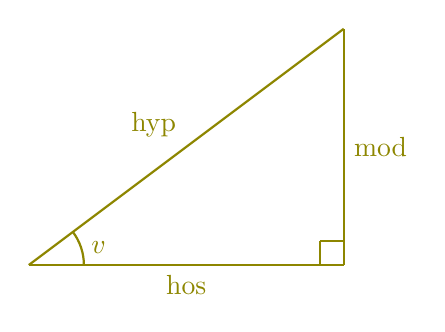
\begin{tikzpicture}
		\draw[color = olive, thick] (0,0) -- (4,0) node[midway, anchor = north] {hos};
		\draw[color = olive, thick] (0,0) -- (4,3) node[midway, anchor = south east] {hyp};
		\draw[color = olive, thick] (4,0) -- (4,3) node[midway, anchor = west] {mod};
		\draw[color = olive, thick] (0.7,0) arc (0:36.87:0.7) node[midway, anchor = west] {$v$};
		\draw[color = olive, thick] (3.7,0) to (3.7,0.3);
		\draw[color = olive, thick] (3.7,0.3) to (4,0.3);
	\end{tikzpicture}
	\caption{Retvinklet trekant.}
	\label{fig:retvinklet}
\end{figure}
Figur \ref{fig:retvinklet} viser os, hvilke sider, vi betegner som hypotenusen (hyp), den modstående katete (mod) og den hosliggende katete (hos.)

Vi husker os selv på følgende sætning fra sidst.
\begin{setn}\label{setn:trigretvinkel}
	For de trigonometriske funktioner $\cos$, $\sin$ og $\tan$ gælder der følgende forhold for sidelængderne i 
	retvinklede trekanter.
	\begin{align*}
		\cos(v) &= \frac{\textnormal{hos}}{\textnormal{hyp}},\\
		\sin(v) &= \frac{\textnormal{mod}}{\textnormal{hyp}},\\
		\tan(v) &= \frac{\textnormal{mod}}{\textnormal{hos}}.
	\end{align*}
\end{setn}
\begin{proof}
	Opgave.
\end{proof}

\section*{Pythagoras' sætning}
\stepcounter{section}

Pythagoras' sætning giver en relation mellem sidelængderne i retvinklede trekanter. Vi betragter trekanten
$\triangle ABC$ på Figur \ref{fig:pytte}.
\begin{figure}[H]
	\centering
	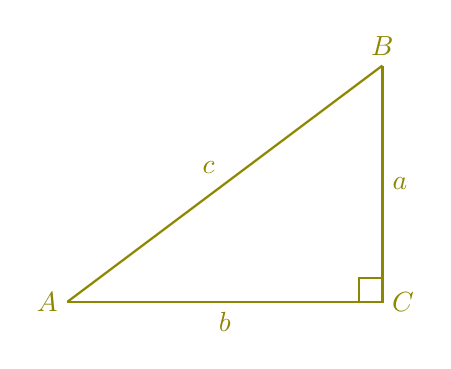
\begin{tikzpicture}
		\draw[color = olive, thick] (0,0) -- (4,0) node[midway, anchor = north] {$b$};
		\draw[color = olive, thick] (0,0) -- (4,3) node[midway, anchor = south east] {$c$};
		\draw[color = olive, thick] (4,0) -- (4,3) node[midway, anchor = west] {$a$};
		\draw[color = olive, thick] (3.7,0) rectangle (4,0.3);
		\node[color = olive, anchor = east] at (0,0) {$A$};
		\node[color = olive, anchor = west] at (4,0) {$C$};
		\node[color = olive, anchor = south] at (4,3) {$B$};
	\end{tikzpicture}
	\caption{Retvinklet trekant.}
	\label{fig:pytte}
\end{figure}
\begin{setn}[Pythagoras]
	For retvinklede trekanter som den, der ses på Figur \ref{fig:pytte} gælder det, at 
	\begin{align*}
		a^2 + b^2 = c^2.
	\end{align*}
\end{setn}
Vi gemmer beviset til senere.
\subsection*{Opgave 1}
Brug hvad du ved om ensvinklede trekanter til at bestemme sidelængderne $a$ og $b$ i følgende trekant:

\begin{center}
	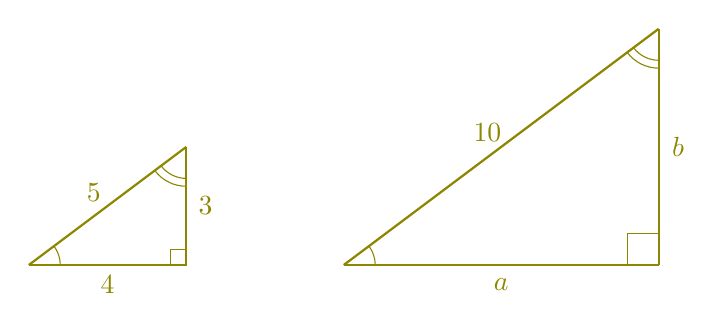
\begin{tikzpicture}
		\draw[color = olive, thick] (-2,0) -- (0,0) node[midway, yshift = -7pt] {4};
		\draw[color = olive, thick] (0,0) -- (0,1.5) node[midway, xshift = 7pt] {3};
		\draw[color = olive, thick] (-2,0) -- (0,1.5) node[midway, yshift = 5pt, xshift = -5pt] {5};
		\draw[color = olive] (0,0) rectangle (-0.2,0.2);
		\draw[color = olive, thick] (2,0) -- (6,0) node[midway, yshift = -7pt] {$a$};
		\draw[color = olive, thick] (6,3) -- (6,0) node[midway, xshift = 7pt] {$b$};
		\draw[color = olive, thick] (2,0) -- (6,3) node[midway, yshift = 5pt,
		xshift = -5pt] {10};
		\draw[color = olive] (6,0) rectangle (5.6,0.4);
		%angle arcs for first triangle
		\draw[color = olive] (-2+.4,0) arc (0:{acos(4/5)}:0.4);
		\draw[color = olive] (0,1.5-0.4) arc (-90:-{acos(3/5)}-90:0.4);
		\draw[color = olive] (0,1.5-0.5) arc (-90:-{acos(3/5)}-90:0.5);
		%angle arcs for second triangle
		\draw[color = olive] (2+.4,0) arc (0:{acos(4/5)}:0.4);
		\draw[color = olive] (6,3-0.4) arc (-90:-{acos(3/5)}-90:0.4);
		\draw[color = olive] (6,3-0.5) arc (-90:-{acos(3/5)}-90:0.5);
	\end{tikzpicture}
\end{center}

\subsection*{Opgave 2}

Vi skal nu bevise Sætning \ref{setn:trigretvinkel}. Vi betragter derfor Figur \ref{fig:bevis}

\begin{figure}[H]
	\begin{center}
	\begin{tikzpicture}
		\begin{axis}[
			axis lines = center, 
			xmin = -1.4, xmax = 3.4, 
			ymin = -1.4, ymax = 3.4, 
			x = 3cm, y = 3cm,
			xtick = {-1.6},
			ytick = {-1.6},
			xlabel = $x$, ylabel = $y$
		]
			%Shifted tick labels since unit circle would otherwise be in the way:
			\node[xshift = 5pt, yshift = -10pt] at (axis cs:1,0) {1};
			\node[xshift = -8pt, yshift = 5pt] at (axis cs:0,1) {1};
			%Circle, lines and angle:
			\draw[color = teal, thick] (axis cs:0,0) circle (3cm);
			\draw[thick, color = teal] (axis cs: 0,0) to (axis cs: {cos(45)},{sin(45)});
			\draw[thick, color = teal] (axis cs: 0.2,0) arc (0:45:0.6cm) node[midway, xshift = 5pt, yshift = 2pt] {$v$};
			\draw[thick, color = teal] (axis cs: {cos(45)},{sin(45)}) to (axis cs: {cos(45)},0);
			\draw[thick, color = teal] (axis cs: 0,0) to (axis cs: {cos(45)},0);
			\draw[color = teal, thick] (axis cs: {cos(45)},0) rectangle (axis cs: {cos(45)-0.1},0.1);
			\draw[color = teal, thick] (axis cs: 0,0) -- (axis cs: 3,0)
			node[midway, yshift = -7pt] {$a$};
			\draw[color = teal, thick] (axis cs: 3,0) -- (axis cs: 3,3) node[midway, xshift = 7pt] {$b$};
			\draw[color = teal, thick] (axis cs: 0,0) -- (axis cs: 3,3) node[midway, yshift = 7pt, xshift = -5pt] {$c$};
			\draw[color = teal, thick] (axis cs: 3,0) rectangle (axis cs: 3-0.1,0.1);
		\end{axis}
	\end{tikzpicture}
	\end{center}
	\caption{To ensvinklede trekanter i et koordinatsystem med enhedscirklen}
	\label{fig:bevis}
\end{figure}

\begin{enumerate}[label=\roman*)]
	\item Tegn Figur \ref{fig:bevis} i jeres gruppe. 
	\item Hvad er længden af hypotenusen for den lille trekant? Skriv det på jeres figur.
	\item Hvad er højden og bredden af den lille trekant? Sammenlign eventuelt med enhedscirklen på Figur \ref{fig:enhed}.
	\item Hvor mange gange større er den store trekant end den lille trekant? Tænk på hvad i gjorde i Opgave 1 (I skal ikke måle, men regne med bogstaver).
 	\item Hvad skal vi gange højden med i den lille trekant for at få $b$? Skriv det udtryk op.
 	\item Hvad skal vi gange bredden med i den lille trekant for at få $a$? Skriv det udtryk op.
	\item Isolér $\sin(v)$ i det første udtryk. 
	\item Isolér $\cos(v)$ i det andet udtryk.  
	\item Hvad er hyp, hos og mod i den store trekant? Indsæt det i de to udtryk. 
	\item Sammenlign jeres resultat med Sætning \ref{setn:trigretvinkel}.
	\item Vi skal nu også vise udtrykket for $\tan(v)$. Tegn derfor endnu en retvinklet trekant, der er lidt større end 
	den lille trekant og hvis lodrette linje går gennem punktet $(1,0)$. 
	\item Hvor høj er denne trekant? Tænk på enhedscirklen fra Figur \ref{fig:enhed}.
	\item Hvad er skalafaktoren mellem denne trekant og den store trekant?
	\item Hvad skal vi gange højden med i den mellemste trekant for at få $a$? Skriv dette udtryk op.
	\item Isolér $\tan(v)$ i dette udtryk.
	\item indsæt igen hyp, hos og mod i udtrykket og sammenlign med Sætning \ref{setn:trigretvinkel}.
\end{enumerate}

\subsection*{Opgave 3}
Bestem de ukendte sider i følgende trekanter.
\begin{center}

\begin{minipage}[t]{0.45\textwidth}
	\centering
	\resizebox{0.95\textwidth}{!}{
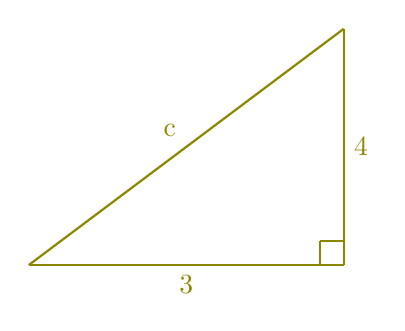
\begin{tikzpicture}
	\draw[color = olive, thick] (0,0) -- (4,0) node[midway, anchor = north] {3};
	\draw[color = olive, thick] (0,0) -- (4,3) node[midway, anchor = south east] {c};
	\draw[color = olive, thick] (4,0) -- (4,3) node[midway, anchor = west] {4};
	\draw[color = olive, thick] (3.7,0) to (3.7,0.3);
	\draw[color = olive, thick] (3.7,0.3) to (4,0.3);
\end{tikzpicture}
}
\end{minipage}%
\hfill
\begin{minipage}[t]{0.45\textwidth}
	\centering
	\resizebox{0.95\textwidth}{!}{
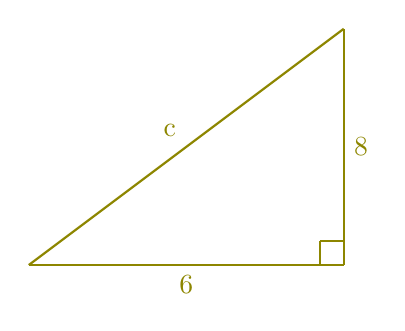
\begin{tikzpicture}
	\draw[color = olive, thick] (0,0) -- (4,0) node[midway, anchor = north] {6};
	\draw[color = olive, thick] (0,0) -- (4,3) node[midway, anchor = south east] {c};
	\draw[color = olive, thick] (4,0) -- (4,3) node[midway, anchor = west] {8};
	\draw[color = olive, thick] (3.7,0) to (3.7,0.3);
	\draw[color = olive, thick] (3.7,0.3) to (4,0.3);
\end{tikzpicture}
}
\end{minipage}%
\hfill
\newpage

\begin{minipage}[t]{0.45\textwidth}
	\centering
	\resizebox{0.95\textwidth}{!}{
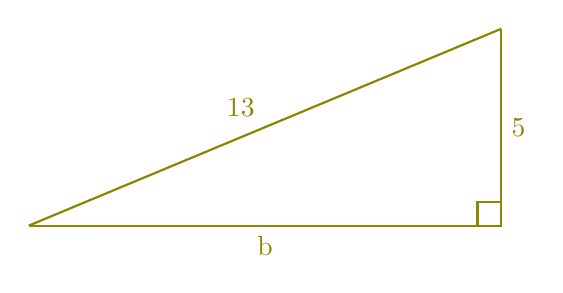
\begin{tikzpicture}
	\draw[color = olive, thick] (0,0) -- (6,0) node[midway, anchor = north] {b};
	\draw[color = olive, thick] (0,0) -- (6,2.5) node[midway, anchor = south east] {13};
	\draw[color = olive, thick] (6,0) -- (6,2.5) node[midway, anchor = west] {5};
	\draw[color = olive, thick] (5.7,0) rectangle (6,0.3);
\end{tikzpicture}
}
\end{minipage}%
\hfill
\begin{minipage}[t]{0.45\textwidth}
	\centering
	\resizebox{0.95\textwidth}{!}{
\begin{tikzpicture}
	\draw[color = olive, thick] (0,0) -- (7.5,0) node[midway, anchor = north] {15};
	\draw[color = olive, thick] (0,0) -- (7.5,4) node[midway, anchor = south east] {17};
	\draw[color = olive, thick] (7.5,0) -- (7.4,4) node[midway, anchor = west] {a};
	\draw[color = olive, thick] (7.2,0) rectangle (7.5,0.3);
\end{tikzpicture}
}
\end{minipage}%
\hfill

\end{center}


\subsection*{Opgave 4}

En retvinklet trekant $\triangle ABC$ med $\angle C = 90^\circ$ opfylder, at $a = 4$ og har desuden et areal på 6.
\begin{enumerate}[label=\roman*)]
	\item Tegn en skitse af trekanten $\triangle ABC$
	\item Bestem sidelængderne $b$ og $c$. 
\end{enumerate}

\subsection*{Opgave 5}
En retvinklet trekant $\triangle ABC$ med $\angle C = 90^\circ$ opfylder, at $b = 7$ og har desuden et areal på 77.
\begin{enumerate}[label=\roman*)]
	\item Tegn en skitse af trekanten $\triangle ABC$
	\item Bestem sidelængderne $a$ og $c$. 
\end{enumerate}

\subsection*{Opgave 6}
To ensvinklede trekanter $\triangle ABC$ og $\triangle PQR$ hvor $\angle C = 90^\circ$ samt $\angle R = 90^\circ$ opfylder, at arealet af $\triangle PQR$ er 54 samt $p = 12$. Skalafaktoren mellem trekanterne er $k = 1.5$ og $\triangle PQR$ er den største af trekanterne. 
\begin{enumerate}[label=\roman*)]
	\item Tegn en skitse af trekanterne $\triangle ABC$ og $\triangle PQR$. 
	\item Bestem sidelængden $q$. 
	\item Bestem sidelængderne $a$, $b$ og $c$. 
	\item Bestem arealet af $\triangle ABC$. 
\end{enumerate}

\newpage
\subsection*{Opgave 7 (med hjælpemidler)}

En trekant $\triangle ABC$ er givet ved følgende figur. Det oplyses, at arealet af trekanten er 10.
\begin{center}
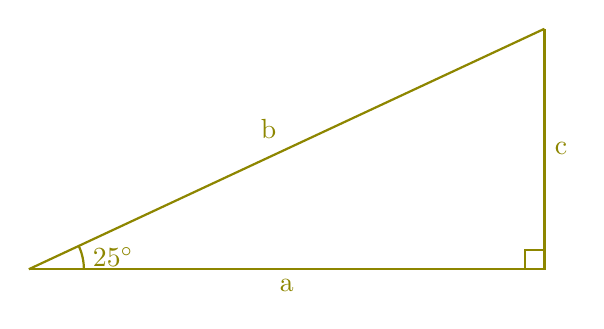
\begin{tikzpicture}
	\draw[color = olive, thick] (0,0) -- (6.5490,0) node[midway, anchor = north] {a};
	\draw[color = olive, thick] (0,0) -- (6.5490,3.053874962) node[midway, anchor = south east] {b};
	\draw[color = olive, thick] (6.5490,0) -- (6.5490,3.053874962) node[midway, anchor = west] {c};
	\draw[color = olive, thick]	(6.3,0) rectangle (6.5490,6.5490-6.3);
	\draw[color = olive, thick] (0.7,0) arc (0:25:0.7) node[midway, anchor = west] {$25^\circ$};
\end{tikzpicture}
\end{center}

\begin{enumerate}[label=\roman*)]
	\item Bestem sidelængderne af trekanten.
\end{enumerate}

\subsection*{Opgave 8 (Med hjælpemidler)}
En \textit{korde} er en ret linje, der forbinder to punkter $P$ og $Q$ på en cirkelperiferi. Vi kan se en korde på Figur \ref{fig:korde}
\begin{figure}[H]
	\centering
	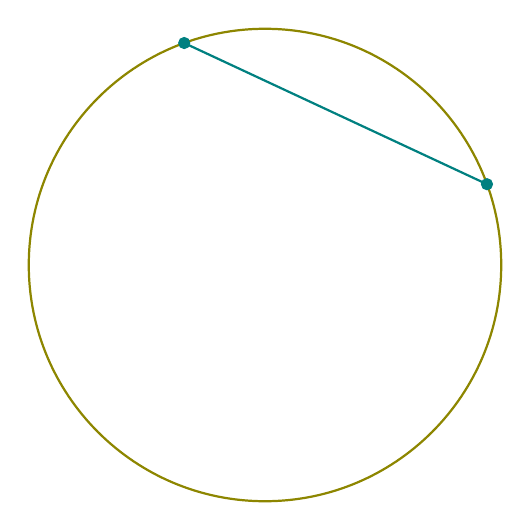
\begin{tikzpicture}
	\draw[color = olive, thick] (0,0) circle (3);
	\filldraw[color = teal] ({3*cos(20)}, {3*sin(20)} ) circle (2pt); 
	\filldraw[color = teal] ({3*cos(110)}, {3*sin(110)} ) circle (2pt); 
	\draw[color = teal, thick] ({3*cos(20)}, {3*sin(20)} ) -- ({3*cos(110)}, {3*sin(110)} );
	\end{tikzpicture}
	\caption{Korde}
	\label{fig:korde}
\end{figure}

En cirkel $C$ har en radius på 5 og en korde med en længde på 8. 
\begin{enumerate}[label=\roman*)]
	\item Bestem længden af det stykke af cirkelbue, korden afgrænser (Vink: kan du lave en retvinklet trekant ved brug
	af radius og korden? Se Figur \ref{fig:kordeopg}.)
\end{enumerate}
\begin{figure}[H]
	\centering
	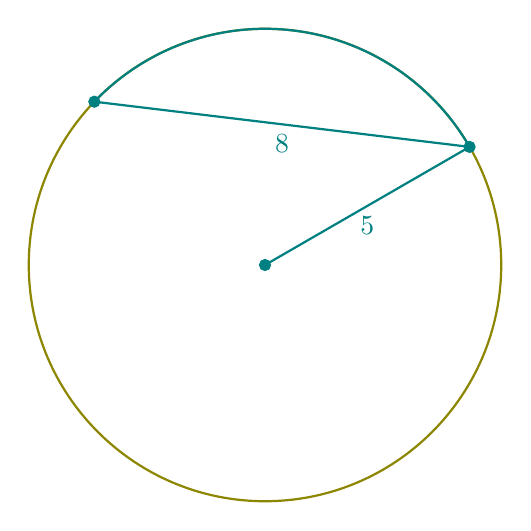
\begin{tikzpicture}
	\draw[color = olive, thick] (0,0) circle (3);
	\filldraw[color = teal] ({3*cos(30)}, {3*sin(30)} ) circle (2pt); 
	\filldraw[color = teal] ({3*cos(30+106.26)}, {3*sin(30+106.26)} ) circle (2pt); 
	\draw[color = teal, thick] ({3*cos(30)}, {3*sin(30)} ) -- ({3*cos(30+106.26)}, {3*sin(30+106.26)} )
	node[midway, anchor = north] {$8$};
	\draw[color = teal, thick] ({3*cos(30)}, {3*sin(30)} ) -- (0,0) node[midway, anchor = north] {$5$};
	\filldraw[color = teal] (0,0) circle (2pt);
	\draw[color = teal, thick] ({3*cos(30)}, {3*sin(30)} ) arc[start angle = 30, end angle = {30+106.26}, radius = 3];
	\end{tikzpicture}
	\caption{Korde med længde 8}
	\label{fig:kordeopg}
\end{figure}

\subsection*{Opgave 9}
Inspireret af den tidligere opgave skal vi bevise, at længden $k$ af en korde i en cirkel med radius $r$ henover en vinkel $\theta$ er givet ved
\begin{align*}
	k = 2r\sin\left(\frac{\theta}{2}\right).
\end{align*}
\begin{enumerate}[label=\roman*)]
	\item Brug Figur \ref{fig:kordebevis} til at bevise formlen for længden af en korde.
\end{enumerate}


\begin{figure}[H]
	\centering
	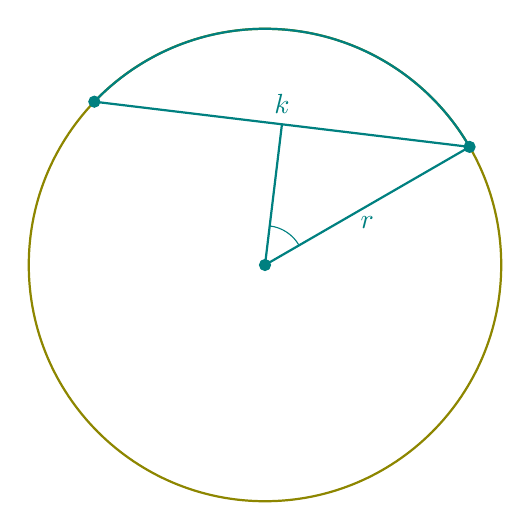
\begin{tikzpicture}
	\draw[color = olive, thick] (0,0) circle (3);
	\filldraw[color = teal] ({3*cos(30)}, {3*sin(30)} ) circle (2pt); 
	\filldraw[color = teal] ({3*cos(30+106.26)}, {3*sin(30+106.26)} ) circle (2pt); 
	\draw[color = teal, thick] ({3*cos(30)}, {3*sin(30)} ) -- ({3*cos(30+106.26)}, {3*sin(30+106.26)} )
	node[midway, anchor = south] {$k$};
	\draw[color = teal, thick] ({3*cos(30)}, {3*sin(30)} ) -- (0,0) node[midway, anchor = north] {$r$};
	\filldraw[color = teal] (0,0) circle (2pt);
	\draw[color = teal, thick] ({3*cos(30)}, {3*sin(30)} ) arc[start angle = 30, end angle = {30+106.26}, radius = 3];
	\draw[color = teal, thick] (0,0) -- ({1.8*cos(30+53.13)},{1.8*sin(30+53.13)});
	\draw[color = teal] ({0.5*cos(30)},{0.5*sin(30)}) arc[start angle = 30, end angle = {30+53.13}, radius = 0.5];
	\end{tikzpicture}
	\caption{Bevis for længde af korde}
	\label{fig:kordebevis}
\end{figure}